\chapter{Introducción}

    En este primer capítulo se explica en líneas generales el tema abordado en el proyecto. Se explica la motivación para la realización de este proyecto, nuestros objetivos y la estructura de este documento.

\section{Motivación}
    Esta memoria de \gls{TFG} tiene como propósito describir el objetivo, desarrollo y funcionamiento de las aplicaciones creadas para este proyecto.
    
    Hoy en día, miles de millones de dispositivos pueden conectarse a internet. Nuestra vida diaria también ha cambiado bastante con una gran cantidad de aplicaciones de IoT o aplicaciones móviles que están basadas en Internet(P.E etiquetas inteligentes, sensores de monitoreo de salud portátiles \enquote{wearables}, automóviles inteligentes, electrodomésticos conectados, etc). Sin embargo, la mayor cantidad de dispositivos conectados y la proliferación de servicios web y multimedia también suponen un gran impacto en la red que podría estar sujeta a mayores incidentes de red. 
    
    La \textbf{telemetría de red} describe cómo se puede recopilar información de varias fuentes de datos utilizando un conjunto de proceso de comunicación automatizados y transmitirlos a los equipos receptores para tareas de análisis. Estas tareas de análisis pueden incluir correlación de eventos, detección de anomalías, monitoreo de rendimiento, análisis de tendencias así como otros procesos relacionados. 
    
    La telemetría de red no supone solo un reto técnico sino también uno comercial. La ejecución exitosa de iniciativas de negocio depende de tener una visión de todas las piezas que componen un sistema. Elementos de almacenamiento, unidades de procesamiento y la infraestructura de transporte en una red son fundamentales para el éxito de las aplicaciones modernas y para una buena experiencia del usuario final. 
    
    \begin{figure}[H]
        \centering
        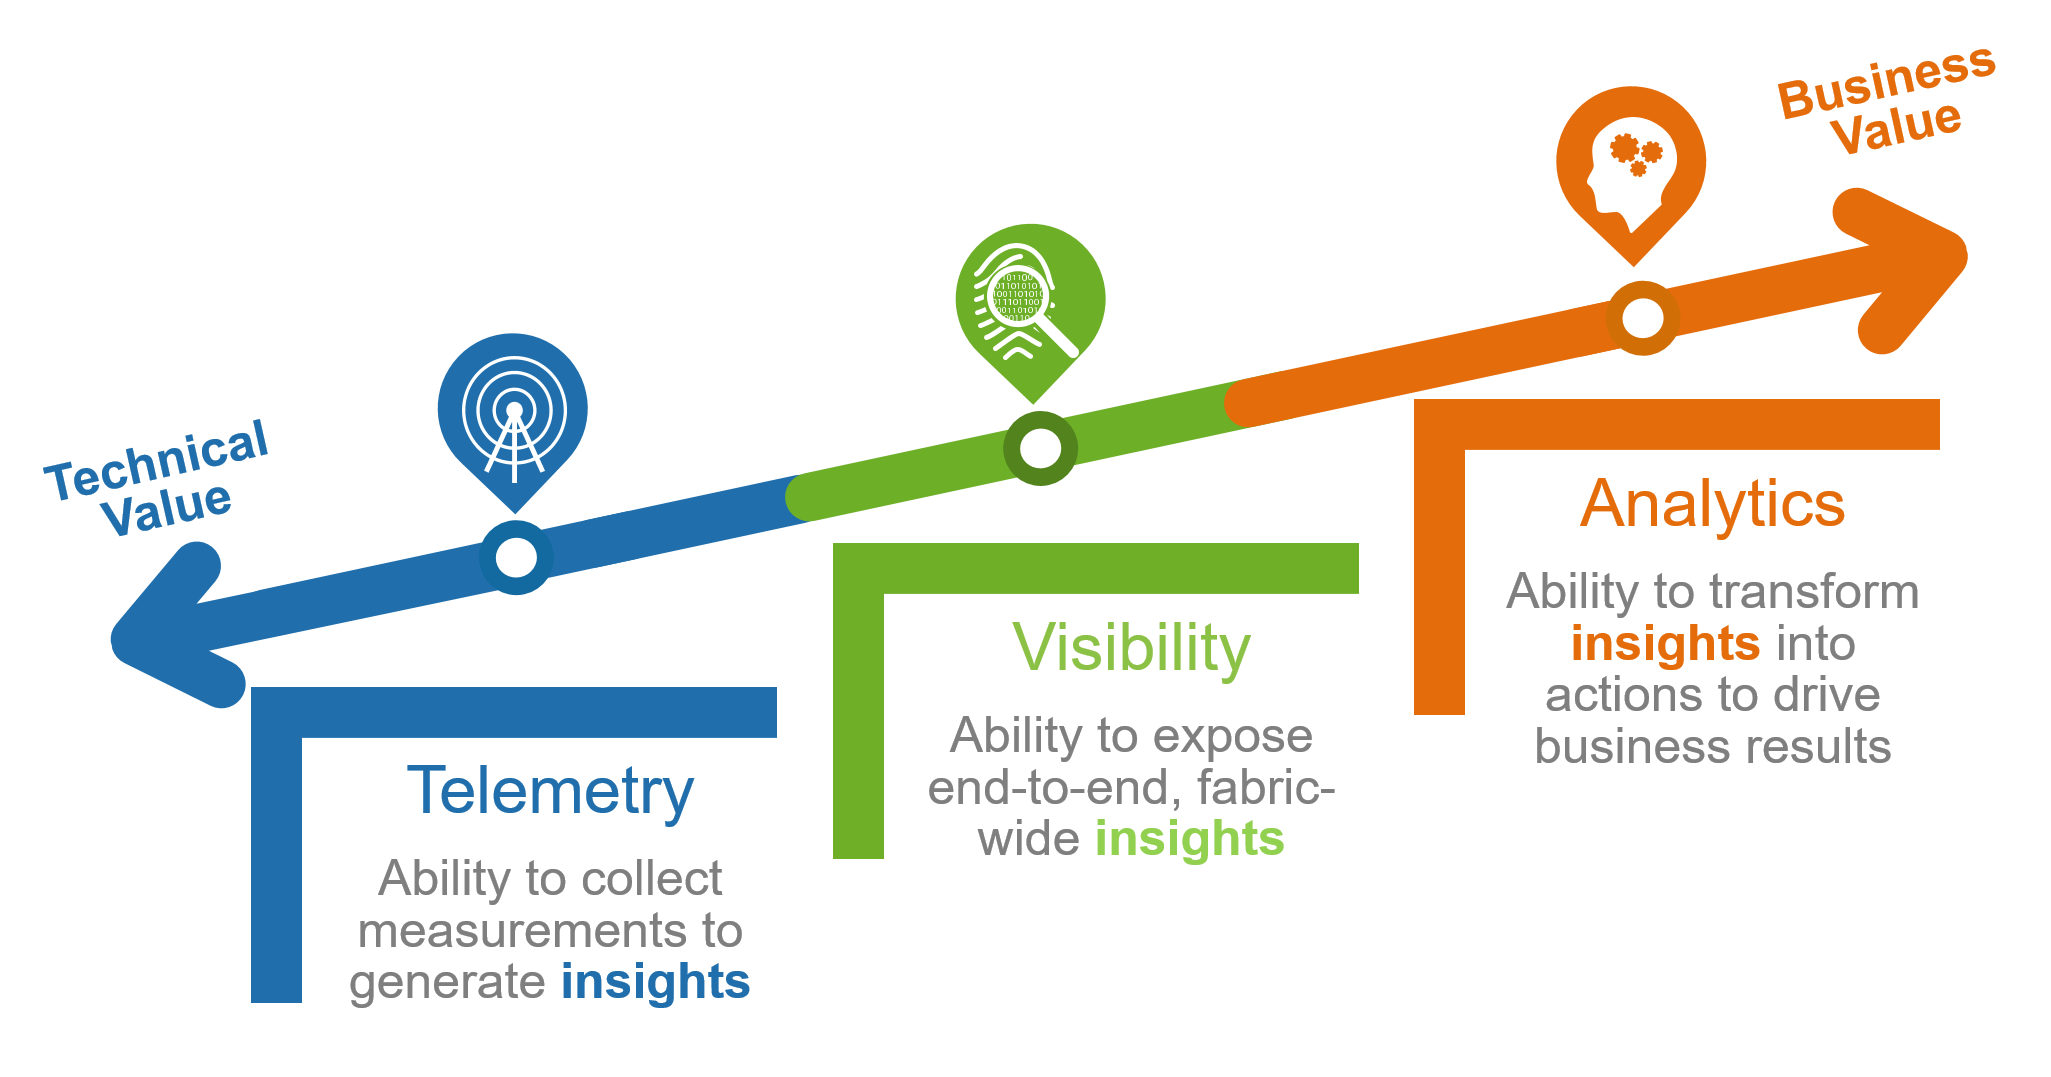
\includegraphics[scale=0.18]{graphics/Telemetry-Visibility-Analytics.png}
        \caption{Network telemetry, visibility and analytics}
        \label{fig:Telemetry_bussinesss}
    \end{figure}
    
    El objetivo de este \gls{TFG} es explorar una de las extensiones del protocolo NETCONF que permitiría el envío de notificaciones y datos de telemetría y desarrollar una implementación que demuestre las capacidades de esta extensión.
    
    El 17 de Abril de 2016 se publica el primer borrador denominado  \enquote{Subscribing to YANG datastore push updates} en el que se empieza a definir los mecanismos de subscripción de tipo \textit{push} para almacenes de datos (\textit{datastores}) que siguen un esquema YANG, que permiten a aplicaciones cliente solicitar notificaciones a un \textit{datastore} YANG que se envían desde un servidor NETCONF en base a una subscripción, sin necesidad de peticiones adicionales enviadas por el cliente\cite{draft-ietf-netconf-yang-push-00}.

    En Septiembre de 2019 tras 25 borradores intermedios se publica el \gls{RFC}8641 en el que se describen los mecanismos que permiten a un cliente solicitar un flujo continuo y personalizado de actualizaciones de un almacén de datos YANG. Estos mecanismos habilitan nuevas capacidades para el monitoreo remoto de la configuración y/o del estado operativo de un dispositivo\cite{RFC8641}.
    
    Junto con este \gls{RFC} la \gls{IETF} trabajó en paralelo desarrollando y completando otras especificaciones como podemos ver en la Figura \ref{fig:telemetry_history}. También podemos observar otros desarrollos por parte de otras organizaciones como OpenConfig y Gooogle (gNMI) que intentan definir su propio modelo para telemetría.
    
    \begin{figure}[H]
        \centering
        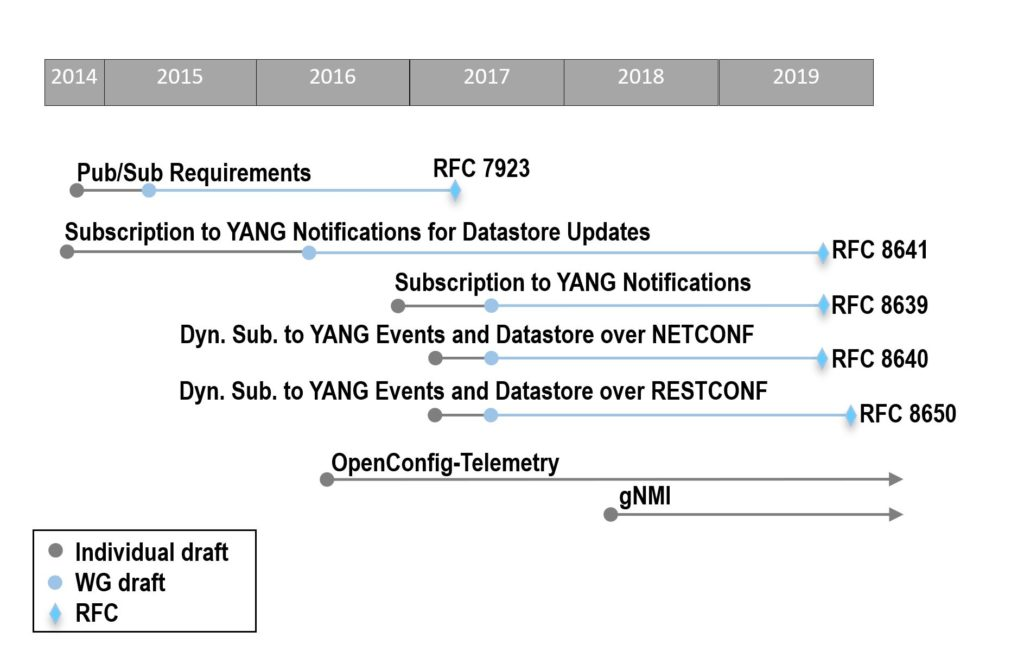
\includegraphics[scale=.5]{graphics/telemetry-history-2-1024x657.jpg}
        \caption{Model-driven Telemetry: Timeline}
        \label{fig:telemetry_history}
    \end{figure}
    
    Este trabajo se centrará en el RFC8641\cite{RFC8641}, que dado que ha sido publicado recientemente, y presenta una oportunidad para estar entre los primeros que implementen y demuestren las capacidades de la extensión definida en dicho \gls{RFC}.

\section{Objetivos}
    Tal como hemos especificado en el apartado anterior nuestro objetivo principal es crear una implementación de la extensión \enquote{Subscription to YANG Notifications for Datastore Updates} para un servidor NETCONF ya existente.

Los objetivos que se buscan alcanzar con el proyecto son los siguientes:

\begin{enumerate}[label=\textbf{O\arabic*} - , leftmargin=3\parindent]

    \item Desarrollar un \textbf{servidor} NETCONF capaz de:
        \begin{enumerate}[label=\textbf{O1.\arabic*} - , leftmargin=1\parindent]
            \item Gestionar notificaciones periódicas.
            \item Gestionar notificaciones de tipo \textit{on-change}.
            \item Soportar filtrado \textit{XPath} y \textit{subtree}
            \item Manejar correctamente los errores e informar a los clientes correctamente.
        \end{enumerate}    
    
    \item Desarrollar un \textbf{cliente} NETCONF que sea capaz de:
        \begin{enumerate}[label=\textbf{O2.\arabic*} - , leftmargin=1\parindent]
            \item Enviar peticiones de subscripción a servidores NETCONF que soporten la extensión de YANG-PUSH.
            \item Enviar modificaciones de subscripciones al servidor NETCONF.
            \item Guardar correctamente los datos enviados por los clientes para su posterior análisis mediante aplicaciones externas.
        \end{enumerate}    
    \item Desarrollar una interfaz para el cliente que permita a un administrador realizar conexiones a servidores, enviar peticiones de subscripción y visualizar los datos recibidos.
\end{enumerate}


\section{Estructura del documento}

Este memoria consta de los siguientes capítulos:
\begin{itemize}
    \item\textbf{Estado del Arte}: Dentro de este capítulo se explicarán cuales son las principales tecnologías y protocolos usados para la gestión de redes.
    \item\textbf{Diseño}: Dentro de este capítulo se explicaran las consideraciones y decisiones de diseño tomadas para cumplir con los objetivos de este proyecto.
    \item\textbf{Desarrollo}: En este capítulo se explicará el funcionamiento interno de la aplicación.
    \item\textbf{Resultados}: Dentro de este capitulo se mostrarán los resultados de las pruebas realizadas y se compararán con los requisitos del RFC8641\cite{RFC8641}.
    \item\textbf{Conclusiones y trabajo futuro}: En este capítulo se presentarán las conclusiones sobre el trabajo realizado y se explorarán posibles desarrollos futuros basados y relacionados con este proyecto. 
\end{itemize}
